\documentclass{jarticle}

\usepackage[dvipdfmx]{graphicx}
\usepackage{float}
\usepackage{url}
\usepackage{caption}

\title{光電効果}
\author{2511198 肥田幸久 \\ 共同実験者 \\ }
\date{2025年10月22日作成}

\begin{document}
\maketitle



\section{実験の目的}

光電管を用いて, 基礎物理定数のひとつであるプランク定数$h$を測定する.
また, 光電効果の諸特性について得られた測定値をもとに検証を行う.



\section{実験の原理}



\subsection{光電効果}

光電効果とは, 金属表面に特定の振動数以上の光が当たると電子(光電子)が飛び出す現象である.
光電子の運動エネルギー$K$と光の振動数$\nu$, 金属表面から光電子が飛び出すのに必要なエネルギー(仕事関数)$W$には, プランク定数$h$を用いて次式の関係が成り立つことが知られている.
\begin{equation}
  K = h\nu - W
\end{equation}

また, 光電効果には次のような性質を持つことが知られている.
\begin{itemize}
  \item 金属の種類によって決まる限界振動数より小さい振動数の光では, 光の強度を強くしても光電子は放出されず, 光の振動数が限界振動数より大きければ, 光の強度がどんなに弱くても光電子は放出される.
  \item 光電子の運動エネルギーは光の強度によらず, 光の振動数にのみ依存する.
  \item 光の振動数を一定にし, その強度を強くしていくと放出される光電子の数が増加するが, 光電子の運動エネルギーは変化しない.
\end{itemize}



\subsection{光電管}

光電管はほぼ真空のガラス管内に入れた陽極と陰極からなり, 光電効果を利用して光エネルギーを電気エネルギーに変換する電子管である.
陰極(光電面)に限界振動数より高い振動数の光を当てると, 飛び出した光電子が陽極へ到達し, 電流として観測することができる.
この電流を光電流と呼び, 陰極には仕事関数が小さいアルカリ金属が用いられる.
これより, 光電管を用いて光電子の運動エネルギーを測定することでプランク定数を求めることができる.
また, 同様の測定を条件を変えて光電流を測定することで上記の光電効果の諸性質を定量的に検証することができる.

光電管には, 光電面から飛び出した光電子を陽極から追い返す向き(逆方向電圧), あるいは加速する向き(順方向電圧)に電圧を変化させながら印加できるようになっている.
光電管に対する印加電圧と陽極より取り出した光電流は各々電圧計と電流計によって測定できる.



\section{実験方法}

本実験では, 以下のような装置を用いて実験を行った.

\begin{figure}[H]
  \begin{center}
    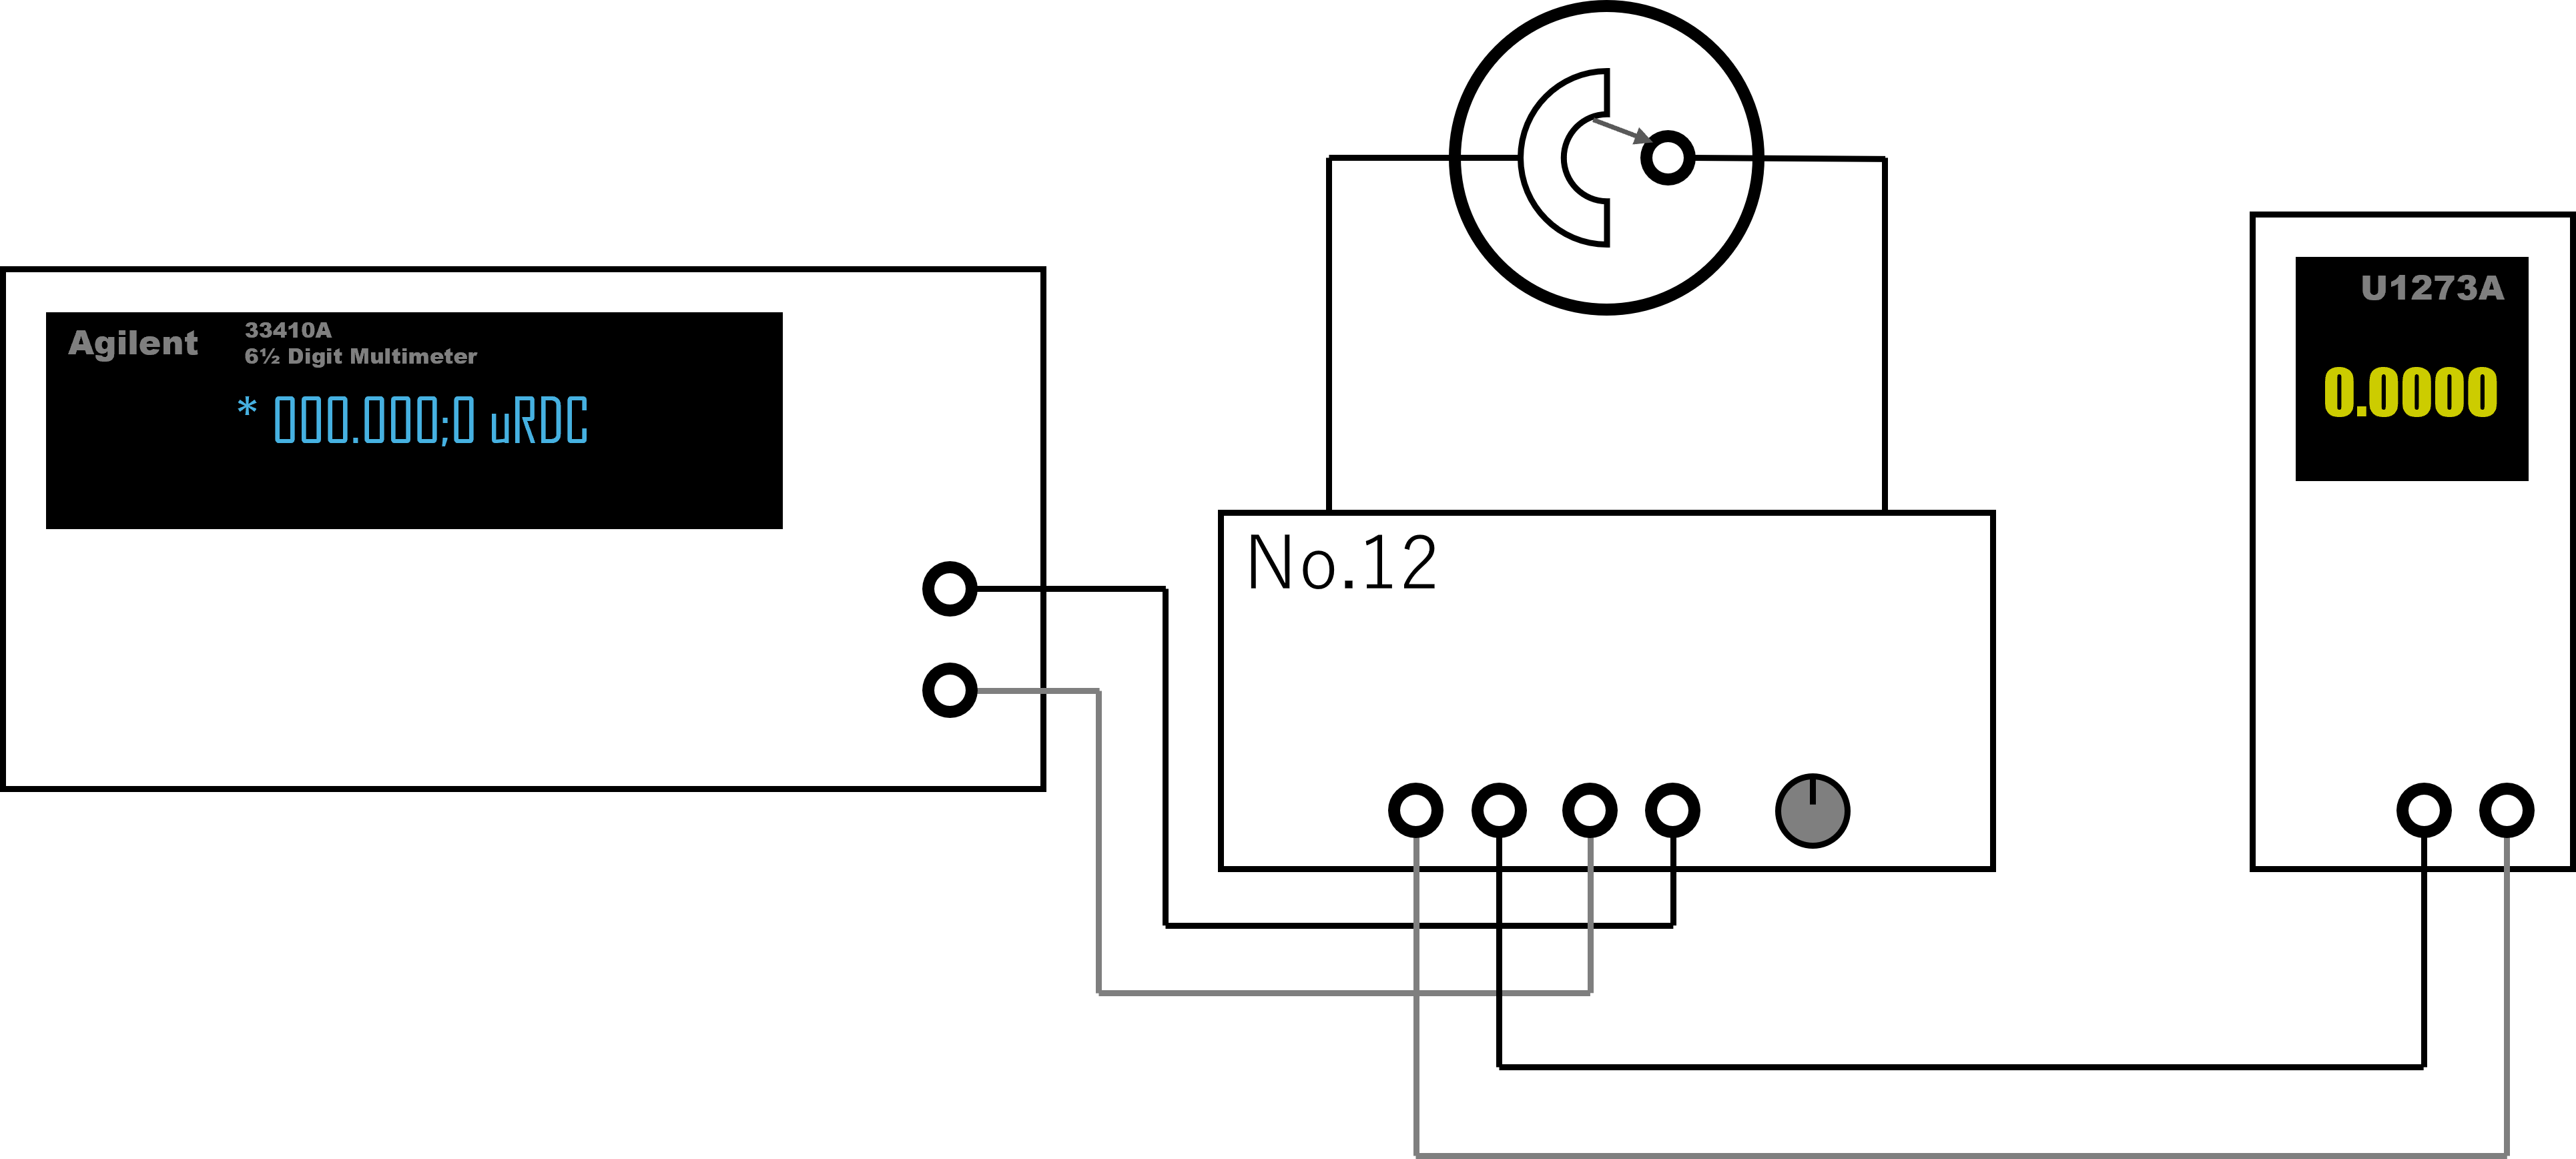
\includegraphics[width=110mm]{picture_experimental_equipment.png}
    \caption{光電効果測定の原理図}
    \label{fg:principle_diagram}
  \end{center}
\end{figure}



\subsection{電流計のオフセット調整}

最初に$7\mathrm{mm}$の絞り板と青色フィルタをセットした.

十分に大きな逆電圧(約$2\mathrm{V}$)を印加し, 光電流を$10$回測定し記録し, 平均値を求めた.
上記をもう一度行い, 平均値に大きな変化がないことを確認し, 表示が平均値近くとなったら$0$補正をした.


\subsection{光電流の測定}

$30\mathrm{nA}$を超えない切りの良い電圧値から光電流の測定を始めた.
その際, $3\mathrm{nA}$以上は$5$回, 未満は$10$回測定した.
$0.05\mathrm{V}$毎に電圧を上げてデータを記録し, 光電流が$1\mathrm{nA}$未満となったら, さらに$3$電圧点ほどまで測定した.
\vskip\baselineskip
以上の操作を, フィルタを変えて繰り返した.



% \subsection{プランク定数$h$と仕事関数$W$の決定}





\section{実験結果}



\subsection{フィルタの波長と振動数}

実験で使用した$4$色のフィルタを通る光の最小の波長$\lambda$と, その振動数$\nu$を表に示す.
ただし, $\nu$の値は光速度$c = 3.0\times 10^8\ \mathrm{m/s}$を用いて計算した.

\begin{table}[H]
  \centering
  \caption{フィルタの波長と振動数}
  \label{tb:wavelength-frequency}
  \begin{tabular}{ccc}
    \hline
    フィルタの色 & 波長$\ \lambda/\mathrm{nm}$ & 振動数$\ \nu/10^{14}\mathrm{Hz}$ \\
    \hline
    赤 & 590 & 5.08 \\
    橙 & 530 & 5.66 \\
    黄 & 492 & 6.10 \\
    青 & 428 & 7.01 \\
    \hline
  \end{tabular}
\end{table}



\subsection{逆電圧に対する光電流の測定結果}



\subsubsection{青色フィルタの場合}

次の表\ref{tb:blue-filter-offset}に, オフセット調整のための, 青色フィルタにおける逆電圧と光電流の測定値を示す.
また, これより$2.0\ I/\mathrm{nA}$でオフセット調整を行った.

\begin{table}[H]
  \caption{青色フィルタにおける電流計のオフセット調整}
  \label{tb:blue-filter-offset}
  \hspace{-2.5cm}
  \begin{tabular}{cccccccccccc}
    \hline
    電圧 & \multicolumn{10}{c}{光電流$\ I/\mathrm{nA}$} & 平均値 \\
    $V/\mathrm{V}$ & 1回目 & 2回目 & 3回目 & 4回目 & 5回目 & 6回目 & 7回目 & 8回目 & 9回目 & 10回目 & $\overline{I}/\mathrm{nA}$ \\
    \hline
    2.0003 & 2.0 & 1.9 & 1.5 & 1.9 & 2.1 & 1.5 & 1.8 & 2.0 & 2.2 & 1.8 & 1.87 \\
    & 1.8 & 2.1 & 1.8 & 1.9 & 2.1 & 2.0 & 1.6 & 2.0 & 2.4 & 1.9 & 1.96 \\
    & 1.9 & 1.7 & 2.0 & 2.1 & 2.0 & 2.1 & 1.8 & 1.9 & 1.9 & 2.0 & 1.94 \\
    \hline
  \end{tabular}
\end{table}

また, 青色フィルタにおける逆電圧と光電流の測定値を次の表\ref{tb:blue-filter}に示す.

\begin{table}[H]
  \caption{青色フィルタにおける逆電圧と光電流の測定値}
  \label{tb:blue-filter}
  \hspace{-2.5cm}
  \begin{tabular}{cccccccccccc}
    \hline
    電圧 & \multicolumn{10}{c}{光電流$\ I/\mathrm{nA}$} & 平均値 \\
    $V/\mathrm{V}$ & 1回目 & 2回目 & 3回目 & 4回目 & 5回目 & 6回目 & 7回目 & 8回目 & 9回目 & 10回目 & $\overline{I}/\mathrm{nA}$ \\
    \hline
    0.0000 & 25.7 & 25.6 & 26.0 & 25.7 & 25.6 & - & - & - & - & - & 25.72 \\
    0.0500 & 22.5 & 22.7 & 22.3 & 22.2 & 22.9 & - & - & - & - & - & 22.52 \\
    0.1000 & 20.1 & 20.2 & 20.1 & 20.1 & 20.1 & - & - & - & - & - & 20.12 \\
    0.1500 & 17.1 & 16.7 & 17.6 & 17.3 & 17.2 & - & - & - & - & - & 17.18 \\
    0.2000 & 14.5 & 14.4 & 14.6 & 14.8 & 14.6 & - & - & - & - & - & 14.58 \\
    0.2500 & 12.3 & 12.1 & 12.2 & 12.4 & 12.8 & - & - & - & - & - & 12.36 \\
    0.3000 & 10.5 & 10.7 & 10.4 & 10.3 & 10.5 & - & - & - & - & - & 10.48 \\
    0.3500 & 8.4 & 8.8 & 8.4 & 8.1 & 8.4 & - & - & - & - & - & 8.42 \\
    0.4000 & 6.6 & 6.9 & 6.7 & 6.4 & 6.7 & - & - & - & - & - & 6.66 \\
    0.4500 & 5.3 & 5.6 & 5.6 & 5.2 & 5.4 & - & - & - & - & - & 5.42 \\
    0.5000 & 4.1 & 3.9 & 4.2 & 4.3 & 4.3 & - & - & - & - & - & 4.16 \\
    0.5500 & 3.1 & 3.2 & 3.1 & 3.2 & 3.0 & - & - & - & - & - & 3.12 \\
    0.6000 & 2.4 & 2.4 & 2.8 & 2.4 & 2.6 & 2.7 & 2.5 & 2.5 & 2.2 & 2.8 & 2.53 \\
    0.6500 & 1.4 & 1.6 & 1.7 & 1.5 & 1.2 & 1.8 & 2.3 & 1.6 & 1.9 & 2.1 & 1.71 \\
    0.7000 & 1.4 & 1.7 & 1.2 & 2.0 & 1.5 & 1.4 & 1.7 & 1.4 & 1.7 & 1.1 & 1.51 \\
    0.7500 & 1.0 & 0.9 & 0.7 & 1.4 & 1.3 & 0.9 & 0.9 & 0.6 & 0.9 & 0.8 & 0.94 \\
    0.8000 & 0.6 & 0.4 & 0.5 & 0.9 & 0.7 & 0.9 & 0.8 & 1.2 & 0.3 & 1.1 & 0.74 \\
    0.8500 & 0.6 & 0.5 & -0.2 & 0.3 & 0.4 & 0.3 & 0.2 & 0.5 & 0.1 & 0.5 & 0.32 \\
    \hline
  \end{tabular}
\end{table}



\subsubsection{黄色フィルタの場合}

次の表\ref{tb:yellow-filter-offset}に, オフセット調整のための, 黄色フィルタにおける逆電圧と光電流の測定値を示す.
また, これより$1.2\ I/\mathrm{nA}$でオフセット調整を行った.

\begin{table}[H]
  \caption{黄色フィルタにおける電流計のオフセット調整}
  \label{tb:yellow-filter-offset}
  \hspace{-2.5cm}
  \begin{tabular}{cccccccccccc}
    \hline
    電圧 & \multicolumn{10}{c}{光電流$\ I/\mathrm{nA}$} & 平均値 \\
    $V/\mathrm{V}$ & 1回目 & 2回目 & 3回目 & 4回目 & 5回目 & 6回目 & 7回目 & 8回目 & 9回目 & 10回目 & $\overline{I}/\mathrm{nA}$ \\
    \hline
    2.0000 & 0.8 & 1.2 & 1.0 & 0.7 & 1.3 & 1.1 & 1.0 & 1.3 & 1.2 & 0.9 & 1.05 \\
    & 1.2 & 1.3 & 1.1 & 1.0 & 1.3 & 1.4 & 1.6 & 1.0 & 1.1 & 1.1 & 1.21 \\
    & 1.2 & 1.4 & 1.3 & 1.4 & 1.6 & 1.5 & 1.4 & 1.4 & 1.6 & 1.3 & 1.41 \\
    & 1.2 & 0.9 & 1.8 & 1.0 & 1.5 & 0.8 & 1.5 & 1.7 & 1.6 & 0.8 & 1.28 \\
    \hline
  \end{tabular}
\end{table}

また, 黄色フィルタにおける逆電圧と光電流の測定値を次の表\ref{tb:yellow-filter}に示す.

\begin{table}[H]
  \caption{黄色フィルタにおける逆電圧と光電流の測定値}
  \label{tb:yellow-filter}
  \hspace{-2.5cm}
  \begin{tabular}{cccccccccccc}
    \hline
    電圧 & \multicolumn{10}{c}{光電流$\ I/\mathrm{nA}$} & 平均値 \\
    $V/\mathrm{V}$ & 1回目 & 2回目 & 3回目 & 4回目 & 5回目 & 6回目 & 7回目 & 8目 & 9回目 & 10回目 & $\overline{I}/\mathrm{nA}$ \\
    \hline
    0.1500 & 36.1 & 36.2 & 36.2 & 36.2 & 35.9 & - & - & - & - & - & 36.12 \\
    0.2001 & 29.0 & 28.0 & 28.2 & 28.7 & 28.4 & - & - & - & - & - & 28.46 \\
    0.2500 & 21.1 & 21.5 & 21.6 & 21.5 & 21.5 & - & - & - & - & - & 21.44 \\
    0.3000 & 15.6 & 16.1 & 15.8 & 15.9 & 16.1 & - & - & - & - & - & 15.90 \\
    0.3500 & 11.3 & 11.1 & 10.8 & 11.2 & 10.8 & - & - & - & - & - & 11.04 \\
    0.4000 & 8.0 & 7.9 & 7.6 & 7.9 & 7.3 & - & - & - & - & - & 7.74 \\
    0.4500 & 5.4 & 5.1 & 5.2 & 5.0 & 5.4 & - & - & - & - & - & 5.22 \\
    0.5001 & 3.0 & 3.1 & 2.8 & 2.9 & 3.2 & - & - & - & - & - & 3.00 \\
    0.5500 & 2.3 & 2.2 & 2.1 & 2.4 & 2.7 & 2.6 & 2.1 & 2.6 & 2.6 & 2.3 & 2.39 \\
    0.6000 & 1.2 & 1.0 & 1.6 & 1.3 & 1.1 & 1.1 & 1.2 & 1.3 & 1.4 & 1.1 & 1.23 \\
    0.6500 & 0.4 & 0.5 & 0.8 & 0.4 & 0.5 & 0.9 & 0.8 & 0.6 & 0.9 & 0.6 & 0.64 \\
    0.7000 & 0.2 & 0.4 & 1.0 & 0.5 & 1.0 & 0.9 & 0.6 & 0.6 & 0.9 & 0.9 & 0.70 \\
    0.7500 & 0.5 & 0.5 & 0.6 & 0.1 & -0.3 & 0.5 & 0.0 & 0.3 & 0.5 & 0.7 & 0.34 \\
    \hline
  \end{tabular}
\end{table}



\subsubsection{橙色フィルタの場合}

次の表\ref{tb:orange-filter-offset}に, オフセット調整のための, 橙色フィルタにおける逆電圧と光電流の測定値を示す.
また, これより$1.2\ I/\mathrm{nA}$でオフセット調整を行った.

\begin{table}[H]
  \caption{橙色フィルタにおける電流計のオフセット調整}
  \label{tb:orange-filter-offset}
  \hspace{-2.5cm}
  \begin{tabular}{cccccccccccc}
    \hline
    電圧 & \multicolumn{10}{c}{光電流$\ I/\mathrm{nA}$} & 平均値 \\
    $V/\mathrm{V}$ & 1回目 & 2回目 & 3回目 & 4回目 & 5回目 & 6回目 & 7回目 & 8回目 & 9回目 & 10回目 & $\overline{I}/\mathrm{nA}$ \\
    \hline
    2.0000 & 1.7 & 1.1 & 1.0 & 1.4 & 1.3 & 1.3 & 1.3 & 1.2 & 1.3 & 0.9 & 1.25 \\
    & 1.2 & 1.3 & 0.7 & 1.3 & 1.3 & 1.4 & 1.1 & 1.3 & 1.1 & 1.4 & 1.21 \\
    \hline
  \end{tabular}
\end{table}

また, 橙色フィルタにおける逆電圧と光電流の測定値を次の表\ref{tb:orange-filter}に示す.

\begin{table}[H]
  \caption{橙色フィルタにおける逆電圧と光電流の測定値}
  \label{tb:orange-filter}
  \hspace{-2.5cm}
  \begin{tabular}{cccccccccccc}
    \hline
    電圧 & \multicolumn{10}{c}{光電流$\ I/\mathrm{nA}$} & 平均値 \\
    $V/\mathrm{V}$ & 1回目 & 2回目 & 3回目 & 4回目 & 5回目 & 6回目 & 7回目 & 8回目 & 9回目 & 10回目 & $\overline{I}/\mathrm{nA}$ \\
    \hline
    0.0000 & 10.7 & 10.6 & 10.4 & 11.1 & 10.8 & - & - & - & - & - & 10.72 \\
    0.0500 & 8.5 & 8.7 & 8.9 & 8.1 & 8.6 & - & - & - & - & - & 8.56 \\
    0.1000 & 6.8 & 6.5 & 6.4 & 6.4 & 7.1 & - & - & - & - & - & 6.64 \\
    0.1500 & 5.0 & 4.9 & 5.3 & 5.5 & 5.1 & - & - & - & - & - & 5.16 \\
    0.2002 & 3.5 & 3.4 & 3.4 & 3.5 & 3.5 & - & - & - & - & - & 3.46 \\
    0.2500 & 1.9 & 2.4 & 2.2 & 2.4 & 2.8 & 2.6 & 2.3 & 2.7 & 2.3 & 2.4 & 2.40 \\
    0.2999 & 2.1 & 1.7 & 1.8 & 2.1 & 2.1 & 2.0 & 2.1 & 1.7 & 1.8 & 1.7 & 1.91 \\
    0.3500 & 1.5 & 1.8 & 1.4 & 1.0 & 1.4 & 1.2 & 1.1 & 1.5 & 1.3 & 0.6 & 1.28 \\
    0.4000 & 0.9 & 0.8 & 0.9 & 1.0 & 1.2 & 0.4 & 1.4 & 0.9 & 0.9 & 1.0 & 0.94 \\
    0.4500 & 0.8 & 0.6 & 1.1 & 0.5 & 0.4 & 0.5 & 0.5 & 0.8 & 0.9 & 0.9 & 0.70 \\
    0.5000 & 0.3 & 0.7 & 0.0 & 0.5 & 0.5 & 0.7 & 0.2 & 0.5 & 0.7 & 0.6 & 0.47 \\
    \hline
  \end{tabular}
\end{table}



\subsubsection{赤色フィルタの場合}

次の表\ref{tb:red-filter-offset}に, オフセット調整のための, 赤色フィルタにおける逆電圧と光電流の測定値を示す.
また, これより$1.2\ I/\mathrm{nA}$でオフセット調整を行った.

\begin{table}[H]
  \caption{赤色フィルタにおける電流計のオフセット調整}
  \label{tb:red-filter-offset}
  \hspace{-2.5cm}
  \begin{tabular}{cccccccccccc}
    \hline
    電圧 & \multicolumn{10}{c}{光電流$\ I/\mathrm{nA}$} & 平均値 \\
    $V/\mathrm{V}$ & 1回目 & 2回目 & 3回目 & 4回目 & 5回目 & 6回目 & 7回目 & 8回目 & 9回目 & 10回目 & $\overline{I}/\mathrm{nA}$ \\
    \hline
    2.0000 & 1.1 & 1.8 & 1.4 & 1.9 & 1.4 & 1.3 & 1.1 & 1.3 & 1.5 & 1.4 & 1.42 \\
    & 1.6 & 1.0 & 1.4 & 1.0 & 1.4 & 0.8 & 1.3 & 1.4 & 1.2 & 1.2 & 1.23 \\
    & 1.3 & 1.2 & 1.2 & 1.4 & 0.8 & 1.2 & 1.4 & 1.0 & 1.3 & 1.3 & 1.21 \\
    \hline
  \end{tabular}
\end{table}

また, 赤色フィルタにおける逆電圧と光電流の測定値を次の表\ref{tb:red-filter}に示す.

\begin{table}[H]
  \caption{赤色フィルタにおける逆電圧と光電流の測定値}
  \label{tb:red-filter}
  \hspace{-2.5cm}
  \begin{tabular}{cccccccccccc}
    \hline
    電圧 & \multicolumn{10}{c}{光電流$\ I/\mathrm{nA}$} & 平均値 \\
    $V/\mathrm{V}$ & 1回目 & 2回目 & 3回目 & 4回目 & 5回目 & 6回目 & 7回目 & 8回目 & 9回目 & 10回目 & $\overline{I}/\mathrm{nA}$ \\
    \hline
    0.0000 & 1.9 & 2.1 & 2.2 & 2.2 & 2.0 & 2.6 & 2.2 & 2.3 & 1.8 & 2.1 & 2.14 \\
    0.0500 & 1.7 & 1.7 & 1.4 & 1.7 & 1.9 & 1.7 & 1.8 & 1.7 & 1.6 & 1.4 & 1.66 \\
    0.1000 & 0.9 & 1.1 & 0.7 & 1.2 & 1.3 & 1.0 & 1.1 & 1.1 & 1.0 & 1.4 & 1.08 \\
    0.1500 & 0.4 & 0.8 & 0.7 & 0.4 & 0.3 & 0.5 & 0.3 & 0.8 & 1.0 & 0.3 & 0.55 \\
    0.2000 & 0.4 & 0.5 & 0.1 & 0.2 & 0.4 & 0.1 & 0.2 & 0.2 & 0.0 & 0.5 & 0.26 \\
    0.2500 & 0.1 & 0.2 & -0.1 & 0.2 & 0.1 & 0.0 & 0.5 & 0.2 & 0.2 & 0.0 & 0.14 \\
    \hline
  \end{tabular}
\end{table}



\subsection{フィルタごとの振動数$\nu$と阻止電圧$V_{th}$の値}

片対数グラフの数$\mathrm{nA}$前後のデータにおおよその直線を引き, $5\ \mathrm{nA}$, $2\ \mathrm{nA}$, $1\ \mathrm{nA}$をよぎる電圧(阻止電圧とする)を求め, 次の表\ref{tb:blocking-voltage}に示す.

\begin{table}[H]
  \centering
  \caption{フィルタごとの振動数$\nu$と阻止電圧$V_{th}$の値}
  \label{tb:blocking-voltage}
  \begin{tabular}{ccccc}
    \hline
    フィルタの色 & 振動数 & \multicolumn{3}{c}{阻止電圧$V_{th}/\mathrm{V}$} \\
    & $\nu/10^{14}\mathrm{Hz}$ & $5\mathrm{nA}$ & $2\mathrm{nA}$ & $1\mathrm{nA}$ \\
    \hline
    赤 & 5.08 & - & 0.015 & 0.078 \\
    橙 & 5.66 & 0.151 & 0.286 & 0.391 \\
    黄 & 6.10 & 0.452 & 0.553 & 0.628 \\
    青 & 7.01 & 0.454 & 0.630 & 0.764 \\
    \hline
  \end{tabular}
\end{table}

更に, 表\ref{tb:blocking-voltage}の値をグラフ上にプロットすると, 図3~6(後掲)のようになった.




\section{考察}



\section{まとめ}



\begin{thebibliography}{99}

  \bibitem{金属の密度} \url{https://www.eng-book.com/sample/pdf/P268.pdf}

\end{thebibliography}

\end{document}